%%%%%%%%%%%%%%%%%%%%%%%%%%%%%%% beamer %%%%%%%%%%%%%%%%%%%%%%%%%%%%%%%%%%%%%%%%%%%%%%%%%
% To run - pdflatex filename.tex
%      acroread filename.pdf
%%%%%%%%%%%%%%%%%%%%%%%%%%%%%%%%%%%%%%%%%%%%%%%%%%%%%%%%%%%%%%%%%%%%%%%%%%%%%%%%%%%%%%%%

\documentclass[compress,oilve]{beamer}
\mode<presentation>

\usetheme[]{CambridgeUS}
% other themes: AnnArbor, Antibes, Bergen, Berkeley, Berlin, Boadilla, boxes, CambridgeUS, Copenhagen, Darmstadt, default, Dresden, Frankfurt, Goettingen,
% Hannover, Ilmenau, JuanLesPins, Luebeck, Madrid, Maloe, Marburg, Montpellier, PaloAlto, Pittsburg, Rochester, Singapore, Szeged, classic

\usecolortheme{beaver}
% color themes: albatross, beaver, beetle, crane, default, dolphin,  fly, lily, orchid, rose, seagull, seahorse, sidebartab, whale, wolverine

\usefonttheme{professionalfonts}
% font themes: default, professionalfonts, serif, structurebold, structureitalicserif, structuresmallcapsserif


\hypersetup{pdfpagemode=FullScreen} % makes your presentation go automatically to full screen

% define your own colors:
\definecolor{Red}{rgb}{1,0,0}
\definecolor{Blue}{rgb}{0,0,1}
\definecolor{Green}{rgb}{0,1,0}
\definecolor{magenta}{rgb}{1,0,.6}
\definecolor{lightblue}{rgb}{0,.5,1}
\definecolor{lightpurple}{rgb}{0.8, 0.6, 0.9}
\definecolor{gold}{rgb}{.6,.5,0}
\definecolor{orange}{rgb}{1,0.4,0}
\definecolor{hotpink}{rgb}{1,0,0.5}
\definecolor{newcolor2}{rgb}{.5,.3,.5}
\definecolor{newcolor}{rgb}{0,.3,1}
\definecolor{newcolor3}{rgb}{1,0,.35}
\definecolor{darkgreen1}{rgb}{0, .35, 0}
\definecolor{darkgreen}{rgb}{0, .6, 0}
\definecolor{darkred}{rgb}{.75,0,0}
\definecolor{skyblue}{HTML}{75bbfd}

\definecolor{olive}{cmyk}{0.64,0,0.95,0.4}
\definecolor{purpleish}{cmyk}{0.75,0.75,0,0}

% can also choose different themes for the "inside" and "outside"

% \usepackage{beamerinnertheme_______}
% inner themes include circles, default, inmargin, rectangles, rounded

% \usepackage{beamerouterthemesmoothbars}
% outer themes include default, infolines, miniframes, shadow, sidebar, smoothbars, smoothtree, split, tree


\useoutertheme[subsection=true, height=40pt]{smoothbars}

% to have the same footer on all slides
%\setbeamertemplate{footline}[text line]{STUFF HERE!}
\setbeamertemplate{footline}[text line]{} % makes the footer EMPTY
% include packages
%

%show the page numbers in footnote
%\addtobeamertemplate{navigation symbols}{}{%
%	\usebeamerfont{footline}%
%	\usebeamercolor[fg]{footline}%
%	\hspace{1em}%
%	\insertframenumber/\inserttotalframenumber
%}

\setbeamercolor{footline}{fg=purpleish}
\setbeamerfont{footline}{series=\bfseries}

%add color to curent subsection
\setbeamertemplate{section in head/foot}{\hfill\tikz\node[rectangle, fill=darkred, rounded corners=1pt,inner sep=1pt,] {\textcolor{white}{\insertsectionhead}};}
\setbeamertemplate{section in head/foot shaded}{\textcolor{darkred}{\hfill\insertsectionhead}}

% Remove bullet of subsections
\setbeamertemplate{headline}
{%
	\begin{beamercolorbox}{section in head/foot}
		\insertsectionnavigationhorizontal{\textwidth}{}{}
	\end{beamercolorbox}%
}


% modify headlline, specially headline size
\setbeamertemplate{headline}{%
	\leavevmode%
	\hbox{%
		\begin{beamercolorbox}[wd=\paperwidth,ht=3.5ex,dp=1.125ex]{palette quaternary}%
			\insertsectionnavigationhorizontal{\paperwidth}{}{\hskip0pt plus1filll}
		\end{beamercolorbox}%
	}
}

\setbeamertemplate{footline}{%
	\leavevmode%
	\hbox{\begin{beamercolorbox}[wd=.5\paperwidth,ht=2.5ex,dp=1.125ex,leftskip=.3cm plus1fill,rightskip=.3cm]{author in head/foot}%
			\usebeamerfont{author in head/foot}\insertshortauthor ~ \insertshortinstitute
		\end{beamercolorbox}%
		\begin{beamercolorbox}[wd=.5\paperwidth,ht=2.5ex,dp=1.125ex,leftskip=.3cm,rightskip=.3cm plus1fil]{title in head/foot}%
			\usebeamerfont{title in head/foot}\insertshorttitle\hfill\insertframenumber\,/\,\inserttotalframenumber
	\end{beamercolorbox}}%
	\vskip0pt%
}


%\setbeamertemplate{navigation symbols}{}

\title{Transformers \& Attention}
\author{ML Instruction Team, Fall 2022}
\institute[]{CE Department \newline  Sharif University of Technology \newline \newline}
\date[\today]{}
%\titlegraphic{\includegraphics[scale=.35]{example-image}}



%Write \usepackage{etex} just after the \documentclass line (it should be the first loaded package).
\usepackage{etex}
\usepackage{subcaption}
\usepackage{multicol}
\usepackage{amsmath}
\usepackage{epsfig}
\usepackage{graphicx}
\usepackage[all,knot]{xy}
\xyoption{arc}
\usepackage{url}
\usepackage{multimedia}
\usepackage{hyperref}
\hypersetup{colorlinks,linkcolor=blue,citecolor=redorange,urlcolor=darkred}
\usepackage{multirow}
\usepackage[font={scriptsize}]{caption}
\usepackage{pgf}
\usepackage{fontspec}
%\setsansfont[Scale=MatchLowercase, BoldFont = * Bold, ItalicFont = * Italic]{Caladea}

%\usepackage{enumitem,xcolor}
%\newcommand{\labelitemi}{$\blacksquare$}
%\newcommand{\labelitemii}{$\diamond$}
%\newcommand{\labelitemiii}{$\square$}
%\newcommand{\labelitemiv}{$\ast$}
%\setbeamercolor*{item}{fg=red}


\usefonttheme{professionalfonts} 
\setbeamertemplate{itemize item}{\color{skyblue}$\blacksquare$}
\setbeamertemplate{itemize subitem}{\color{hotpink}$\blacktriangleright$}
\setbeamertemplate{itemize subsubitem}{\color{orange}$\bullet$}


\usepackage{anyfontsize}
\usepackage{t1enc}
\usepackage{tikz}
\usetikzlibrary{calc,trees,positioning,arrows,chains,shapes.geometric,decorations.pathreplacing,decorations.pathmorphing,shapes,matrix,shapes.symbols}



\newtheorem{proposition}[theorem]{Proposition}
\newtheorem{remark}[theorem]{Remark}
\newtheorem{assumption}[theorem]{Assumption}

\usepackage{xcolor}
\newcommand{\tc}[2]{
	\textcolor{#1}{#2}
}

%\usepackage{fontspec, unicode-math}
%\setmainfont[Scale=0.9]{Nimbus Roman No9 L}
%\setmonofont[Scale=0.9]{Monaco}
\setsansfont[Scale=1]{Times New Roman}

\newcommand{\vect}[1]{\boldsymbol{#1}}

\definecolor{strings}{rgb}{.624,.251,.259}
\definecolor{keywords}{rgb}{.224,.451,.686}
\definecolor{comment}{rgb}{.322,.451,.322}


%\usepackage{smartdiagram}
%\usesmartdiagramlibrary{additions}
%%%%%%%%%%%%%%%%%%%%%%%%%%%%%%%%%%%%%%%%%%%%%%%%%%%%%%%%%%%%%%%%%%%%%%%%%%%%%%%%%%%%%%%%%%%%
%%%%%%%%%%%%%%%%%%%%%%%%%%%%%% Title Page Info %%%%%%%%%%%%%%%%%%%%%%%%%%%%%%%%%%%%%%%%%%%
%%%%%%%%%%%%%%%%%%%%%%%%%%%%%%%%%%%%%%%%%%%%%%%%%%%%%%%%%%%%%%%%%%%%%%%%%%%%%%%%%%%%%%%%%%


%%%%%%%%%%%%%%%%%%%%%%%%%%%%%%%%%%%%%%%%%%%%%%%%%%%%%%%%%%%%%%%%%%%%%%%%%%%%%%%%%%%%%%%%%%
%%%%%%%%%%%%%%%%%%%%%%%%%%%%%% Begin Your Document %%%%%%%%%%%%%%%%%%%%%%%%%%%%%%%%%%%%%%%
%%%%%%%%%%%%%%%%%%%%%%%%%%%%%%%%%%%%%%%%%%%%%%%%%%%%%%%%%%%%%%%%%%%%%%%%%%%%%%%%%%%%%%%%%%
\begin{document}
	
%%%%%%%%%%%%%%%%%%%%%%%%%%%%%%%%%%%%%%%%%%%%%%%%%%%%%%%%%%%%%%%%%%%%%%%%%%%%%%%%%%%%%%%%%%
	\fontsize{9}{9}
\begin{frame}[noframenumbering, plain]
	\titlepage
\end{frame}

%%%%%%%%%%%%%%%%%%%%%%%%%%%%%%%%%%%%%%%%%%%%%%%%%%%%%%%%%%%%%%%%%%%%%%%%%%%%%%%%%%%%%%%%%%
\section{Transformers \& Attention}
%%%%%%%%%%%%%%%%%%%%%%%%%%%%%%%%%%%%%%%%%%%%%%%%%%%%%%%%%%%%%%%%%%%%%%%%######
\frame{\frametitle{Overview}
	
	
\begin{itemize}
	\item 
 
         There has been an array of Transformer based architectures such as BERT, SpanBERT, Transformer-XL, XLNet, GPT-2, etc getting released frequently for the past couple of years.

	\item \vspace{20pt}
         The OpenAI’s GPT-3 had taken the internet by storm with its ability to perform extremely well on tasks such as Q&A, Comprehension, even Programming
	
	\item \vspace{20pt}
	
	But all of this started with a research paper released back in 2017 \href{https://arxiv.org/abs/1706.03762}{"Attention is all you need".}
 
\end{itemize}	
	
}

%%%%%%%%%%%%%%%%%%%%%%%%%%%%%%%%%%%%%%%%%%%%%%%%%%%%%%%%%%%%%%%%%%%%%%%%%%%%%%%%%%%%%%%%%%%%%%%
\frame{\frametitle{What is a Transformer}
	
	
\begin{itemize}
	\item 
 
         They take a text sequence as input and produce another text sequence as output. eg. to translate an input English sentence to Spanish.

	\item \vspace{10pt}
         At its core, it contains a stack of Encoder layers and Decoder layers.
         
\end{itemize}	

\begin{figure}
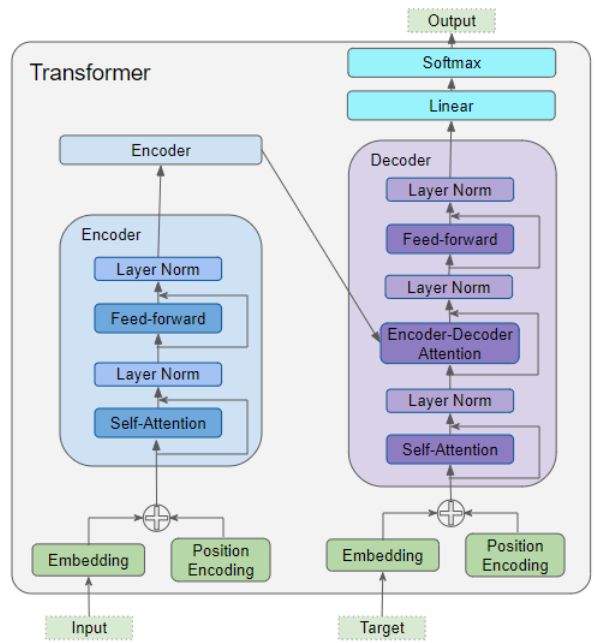
\includegraphics[scale=.4]{Figs/Transformer.png}
\caption{Transformer schematic, \href{https://towardsdatascience.com/transformers-explained-visually-part-2-how-it-works-step-by-step-b49fa4a64f34}{Source}.}
\label{fig:boat1}
\end{figure}
}
%%%%%%%%%%%%%%%%%%%%%%%%%%%%%%%%%%%%%%%%%%%%%%%%%%%%%%%%%%%%%%%%%%%%%%%%%%%%%%%%%%%%%%%%%%%%%%%
\frame{


\begin{itemize}
        \item
        As we can observe in the above figure:

        \begin{itemize}
    	\item 
            The Encoder contains the all-important Self-attention layer that computes the relationship between different words in the sequence, as well as a Feed-forward layer.
    
    	\item \vspace{2pt}
            The Decoder contains the Self-attention layer and the Feed-forward layer, as well as a second Encoder-Decoder attention layer.
    
            \item \vspace{2pt}
            Each Encoder and Decoder has its own set of weights.
        \end{itemize}

        \item \vspace{5pt}
        The Embedding layer encodes the meaning of the word.

        \item \vspace{5pt}
        The Position Encoding layer represents the position of the word.
         
	
 
\end{itemize}	
	
}

%%%%%%%%%%%%%%%%%%%%%%%%%%%%%%%%%%%%%%%%%%%%%%%%%%%%%%%%%%%%%%%%%%%%%%%%%%%%%%%%%%%%%%%%%%%%%%%
\frame{\frametitle{What Does Attention Do ?}
	
	
\begin{itemize}
	\item 
 
         The key to the Transformer’s ground-breaking performance is its use of Attention.

	\item \vspace{7pt}
         While processing a word, Attention enables the model to focus on other words in the input that are closely related to that word. 
         
         \item \vspace{7pt}
	eg. ‘Ball’ is closely related to ‘blue’ and ‘holding’. On the other hand, ‘blue’ is not        related to ‘boy’.
        \begin{figure}
          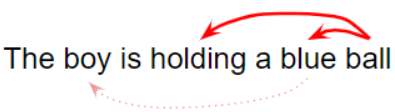
\includegraphics[scale=.4]{Figs/Example.png}
          \label{fig:boat1}
        \end{figure}
        
        \item \vspace{7pt}
        The Transformer architecture uses self-attention by relating every word in the input sequence to every other word. eg. Consider two sentences:
        \begin{itemize}
	\item
            The cat drank the milk because\tc{keywords}{it}was hungry. 
        \item
        The cat drank the milk because\tc{keywords}{it}was sweet.
        \end{itemize}

 
\end{itemize}	
	
}

%%%%%%%%%%%%%%%%%%%%%%%%%%%%%%%%%%%%%%%%%%%%%%%%%%%%%%%%%%%%%%%%%%%%%%%%%%%%%%%%%%%%%%%%%%%%%%%
\frame{
	
	
\begin{itemize}
	\item 
        When the model processes the word 'it', self-attention gives the model more information about its meaning so that it can associate 'it' with the correct word.
        
\end{itemize}

\begin{figure}
  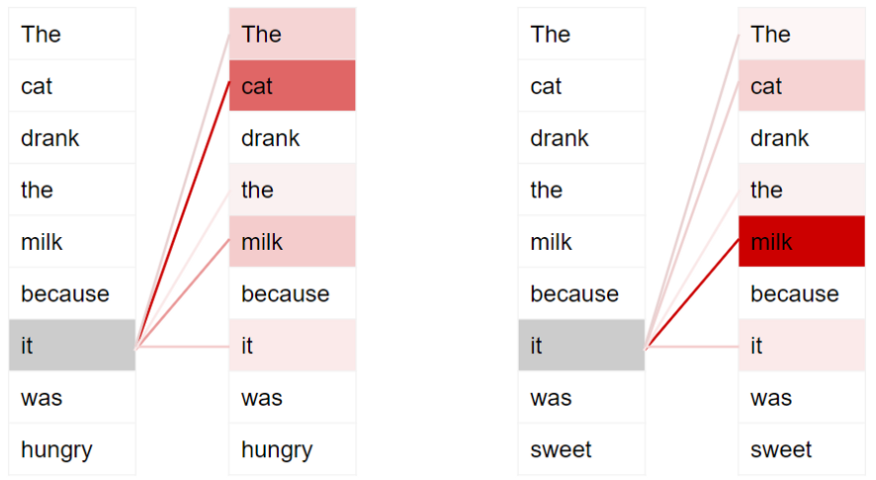
\includegraphics[scale=.4]{Figs/Self-Attention-example.png}
  \caption{Implementation of self attention on the example, \href{https://towardsdatascience.com/transformers-explained-visually-part-1-overview-of-functionality-95a6dd460452}{Source}.}
  \label{fig:Self-Attention-example}
\end{figure}

\begin{itemize}
	\item 
        To enable it to handle more nuances about the intent and semantics of the sentence, Transformers include multiple attention scores for each word. For instance:
\end{itemize}

	
}

%%%%%%%%%%%%%%%%%%%%%%%%%%%%%%%%%%%%%%%%%%%%%%%%%%%%%%%%%%%%%%%%%%%%%%%%%%%%%%%%%%%%%%%%%%%%%%%
\frame{
	
\begin{figure}
  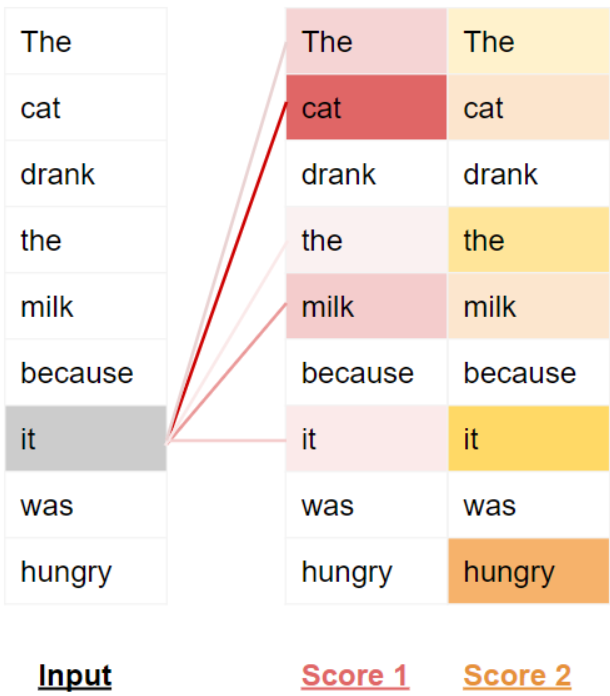
\includegraphics[scale=.4]{Figs/Self-Attention-example2.png}
  \caption{Including multiple attention scores for the same example, \href{https://towardsdatascience.com/transformers-explained-visually-part-1-overview-of-functionality-95a6dd460452}{Source}.}
  \label{fig:Self-Attention-example}
\end{figure}
	
}

%%%%%%%%%%%%%%%%%%%%%%%%%%%%%%%%%%%%%%%%%%%%%%%%%%%%%%%%%%%%%%%%%%%%%%%%%%%%%%%%%%%%%%%%%%%%%%%
\frame{\frametitle{Evolution of Attention}
	
	
\begin{itemize}
	\item 
 
        \tc{keywords}{Version 0}
        
        \begin{itemize}
	\item 
        To understand the intuition of attention, we start with an\tc{keywords}{input}and a\tc{keywords}{query}.
        
        \item \vspace{2pt}
        In terms of computation,\tc{keywords}{attention is given}to parts of the input matrix which is\tc{keywords}{similar}to the query vector.

        \item \vspace{2pt}
        $f_{att}$ which is a 'feed-forward network'. The feed-forward network takes the query and input, and projects both of them to dimension $D_E$.
        \end{itemize}

\end{itemize}	

\vspace{5pt}
\begin{figure}
% \centering
\subfloat[Schematic of attention Version 0, \href{https://pyimagesearch.com/2022/09/05/a-deep-dive-into-transformers-with-tensorflow-and-keras-part-1/}{Source}]{{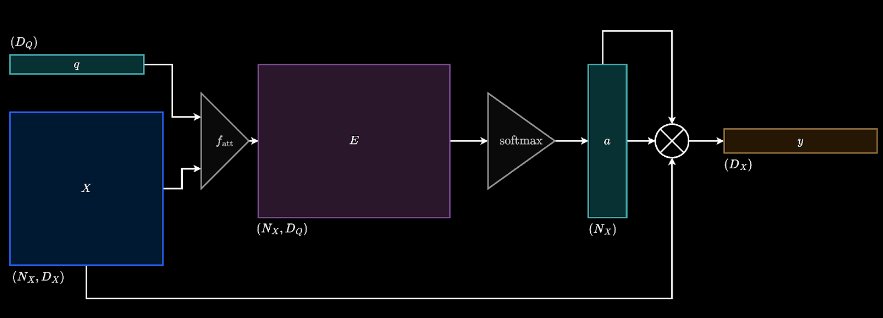
\includegraphics[scale=.3]{Figs/Version 0.png} }}%
\subfloat[Outputs Table, \href{https://pyimagesearch.com/2022/09/05/a-deep-dive-into-transformers-with-tensorflow-and-keras-part-1/}{Source}]{{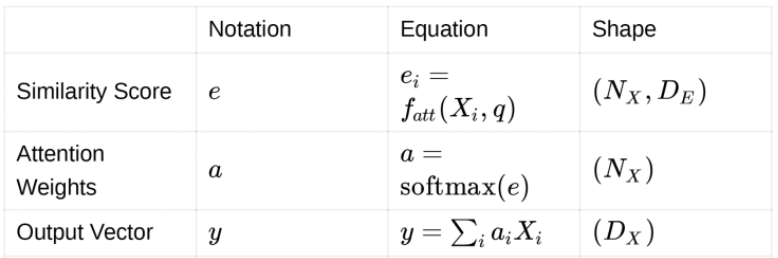
\includegraphics[scale=.3]{Figs/Version 0 Table.png} }}%
\label{FIG:2}
\end{figure}
}

%%%%%%%%%%%%%%%%%%%%%%%%%%%%%%%%%%%%%%%%%%%%%%%%%%%%%%%%%%%%%%%%%%%%%%%%%%%%%%%%%%%%%%%%%%%%%%%
\frame{
	
	
\begin{itemize}
	\item 
 
        \tc{keywords}{Version 1}
        
        \begin{itemize}
	\item 
        The first change we make to the mechanism is swapping out the feed-forward network with a\tc{keywords}{dot product}operation.
        
        \item \vspace{2pt}
        Turns out that this is\tc{keywords}{highly efficient}with reasonably good results.

        \end{itemize}

\end{itemize}	

\vspace{5pt}
\begin{figure}
% \centering
\subfloat[Schematic of attention Version 1, \href{https://pyimagesearch.com/2022/09/05/a-deep-dive-into-transformers-with-tensorflow-and-keras-part-1/}{Source}]{{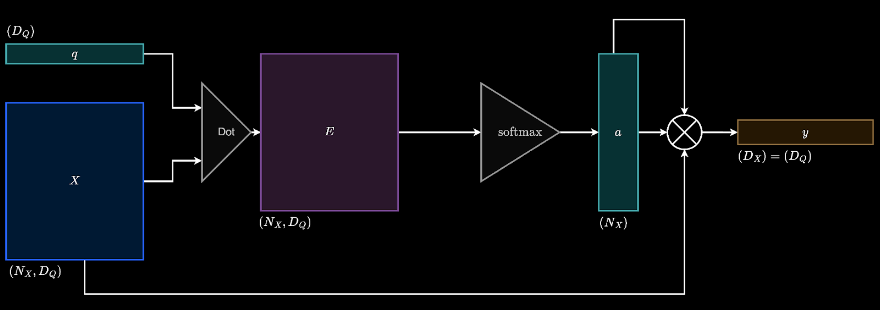
\includegraphics[scale=.3]{Figs/Version 1.png} }}%
\subfloat[Outputs Table, \href{https://pyimagesearch.com/2022/09/05/a-deep-dive-into-transformers-with-tensorflow-and-keras-part-1/}{Source}]{{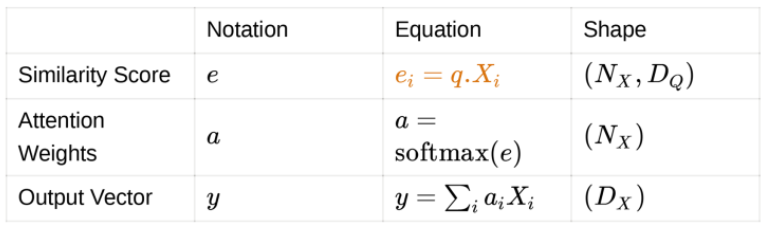
\includegraphics[scale=.3]{Figs/Version 1 Table.png} }}%
\label{FIG:2}
\end{figure}
}

%%%%%%%%%%%%%%%%%%%%%%%%%%%%%%%%%%%%%%%%%%%%%%%%%%%%%%%%%%%%%%%%%%%%%%%%%%%%%%%%%%%%%%%%%%%%%%%
\frame{
	
	
\begin{itemize}
	\item 
 
        \tc{keywords}{Version 2}
        
        \begin{itemize}
	\item 
        This version is a very important concept realized in the original paper. The authors propose\tc{keywords}{scaled dot product}instead of\tc{keywords}{normal dot product}as the similarity function.
        
        \item \vspace{2pt}
        This little change can solve many challenges such as\tc{keywords}{Vanishing Gradient Problem}and Unnormalized softmax.

        \end{itemize}

\end{itemize}	

\vspace{5pt}
\begin{figure}
% \centering
\subfloat[Schematic of attention Version 2, \href{https://pyimagesearch.com/2022/09/05/a-deep-dive-into-transformers-with-tensorflow-and-keras-part-1/}{Source}]{{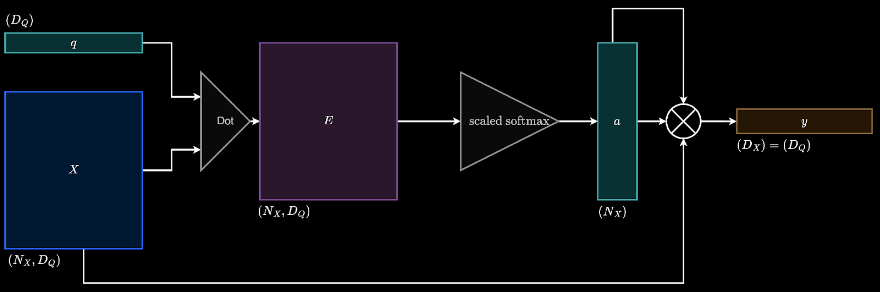
\includegraphics[scale=.3]{Figs/Version 2.png} }}%
\subfloat[Outputs Table, \href{https://pyimagesearch.com/2022/09/05/a-deep-dive-into-transformers-with-tensorflow-and-keras-part-1/}{Source}]{{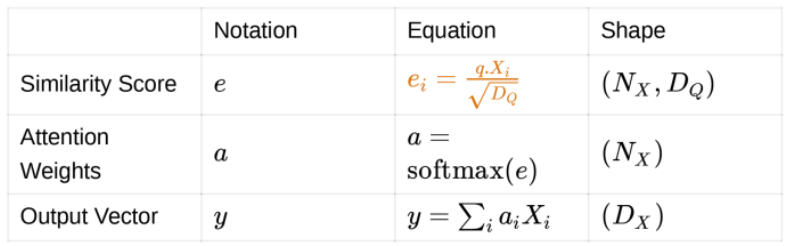
\includegraphics[scale=.3]{Figs/Version 2 Table.png} }}%
\label{FIG:2}
\end{figure}
}

%%%%%%%%%%%%%%%%%%%%%%%%%%%%%%%%%%%%%%%%%%%%%%%%%%%%%%%%%%%%%%%%%%%%%%%%%%%%%%%%%%%%%%%%%%%%%%%
\frame{
	
	
\begin{itemize}
	\item 
 
        \tc{keywords}{Version 3}
        
        \begin{itemize}
	\item 
        Previously we looked at a single query vector. Here we scale this implementation to\tc{keywords}{multiple query}vectors.
        
        \item \vspace{2pt}
        We calculate the similarities of the input matrix with all the query vectors (query matrix) we have.

        \end{itemize}

\end{itemize}	

\vspace{5pt}
\begin{figure}
% \centering
\subfloat[Schematic of attention Version 3, \href{https://pyimagesearch.com/2022/09/05/a-deep-dive-into-transformers-with-tensorflow-and-keras-part-1/}{Source}]{{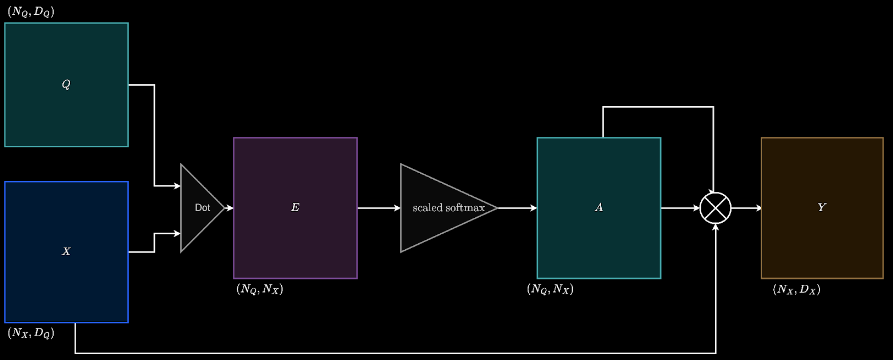
\includegraphics[scale=.3]{Figs/Version 3.png} }}%
\subfloat[Outputs Table, \href{https://pyimagesearch.com/2022/09/05/a-deep-dive-into-transformers-with-tensorflow-and-keras-part-1/}{Source}]{{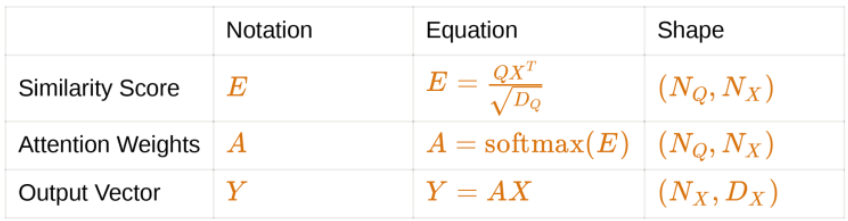
\includegraphics[scale=.3]{Figs/Version 3 Table.png} }}%
\label{FIG:2}
\end{figure}
}

%%%%%%%%%%%%%%%%%%%%%%%%%%%%%%%%%%%%%%%%%%%%%%%%%%%%%%%%%%%%%%%%%%%%%%%%%%%%%%%%%%%%%%%%%%%%%%%
\frame{
	
	
\begin{itemize}
	\item 
 
        \tc{keywords}{Version 4 (Cross-Attention)}
        
        \begin{itemize}
	\item 
        To build cross-attention, we make some changes. The changes are specific to the input matrix. As we already know, attention needs an input matrix and a query matrix.
        
        \item \vspace{2pt}
        Suppose we projected the input matrix into a pair of matrices, namely the\tc{keywords}{key}and\tc{keywords}{value}matrices.

        \item \vspace{2pt}
        This is done to\tc{keywords}{decouple}the complexity. The input matrix can now have a better projection that takes care of building attention weights and better output matrices as well.

        \end{itemize}

\end{itemize}	
\vspace{5pt}
\begin{figure}
% \centering
\subfloat[Schematic of attention Version 4, \href{https://pyimagesearch.com/2022/09/05/a-deep-dive-into-transformers-with-tensorflow-and-keras-part-1/}{Source}]{{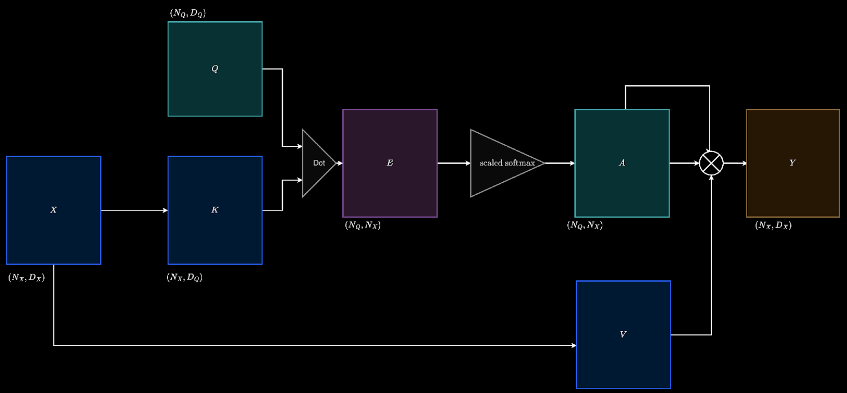
\includegraphics[scale=.3]{Figs/Version 4.png} }}%
\subfloat[Outputs Table, \href{https://pyimagesearch.com/2022/09/05/a-deep-dive-into-transformers-with-tensorflow-and-keras-part-1/}{Source}]{{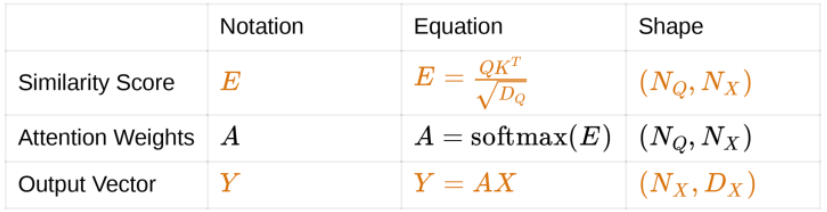
\includegraphics[scale=.3]{Figs/Version 4 Table.png} }}%
\label{FIG:2}
\end{figure}
}

%%%%%%%%%%%%%%%%%%%%%%%%%%%%%%%%%%%%%%%%%%%%%%%%%%%%%%%%%%%%%%%%%%%%%%%%%%%%%%%%%%%%%%%%%%%%%%%
\frame{
	
	
\begin{itemize}
	\item 
 
        \tc{keywords}{Version 5 (Self-Attention)}
        
        \begin{itemize}
	\item 
        Like the Version 4 that the key and value matrix are projected versions of the input matrix. What if the query matrix also was projected from the input?
        
        \item \vspace{2pt}
        Here the main motivation is to build a richer implementation of self with respect to self. This sounds funny, but it is highly important and forms the basis of the Transformer architecture.

        \end{itemize}

\end{itemize}	

\vspace{5pt}
\begin{figure}
% \centering
\subfloat[Schematic of attention Version 5, \href{https://pyimagesearch.com/2022/09/05/a-deep-dive-into-transformers-with-tensorflow-and-keras-part-1/}{Source}]{{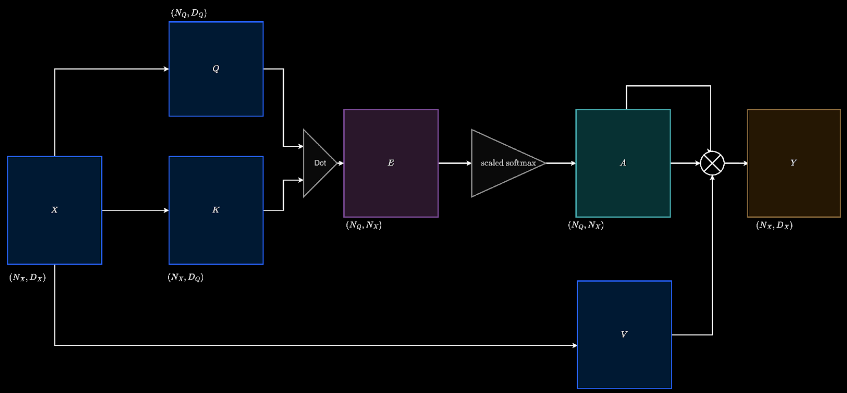
\includegraphics[scale=.3]{Figs/Version 5.png} }}%
\subfloat[Outputs Table, \href{https://pyimagesearch.com/2022/09/05/a-deep-dive-into-transformers-with-tensorflow-and-keras-part-1/}{Source}]{{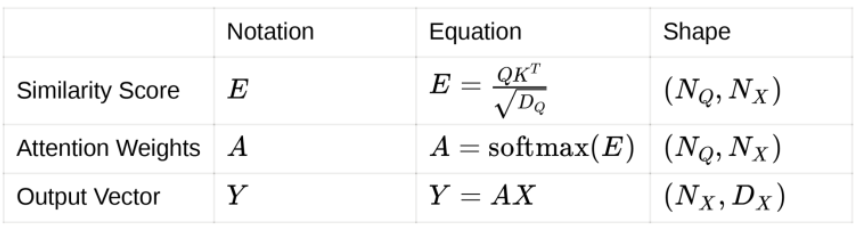
\includegraphics[scale=.3]{Figs/Version 5 Table.png} }}%
\label{FIG:2}
\end{figure}
}

%%%%%%%%%%%%%%%%%%%%%%%%%%%%%%%%%%%%%%%%%%%%%%%%%%%%%%%%%%%%%%%%%%%%%%%%%%%%%%%%%%%%%%%%%%%%%%%
\frame{\frametitle{Training the Transformer}
	
	
\begin{itemize}
        
	\item 
         Training data consists of two parts:
         
        \begin{itemize}
	\item 
        The source or input sequence (eg. 'You are welcome' in English, for a translation problem).
        \item
        The destination or target sequence (eg. 'De nada' in Spanish).
        \end{itemize}
        
        \item \vspace{2pt}
        The Transformer's goal is to learn how to output the target sequence, by using both the input and target sequence.

\end{itemize}	

\begin{figure}
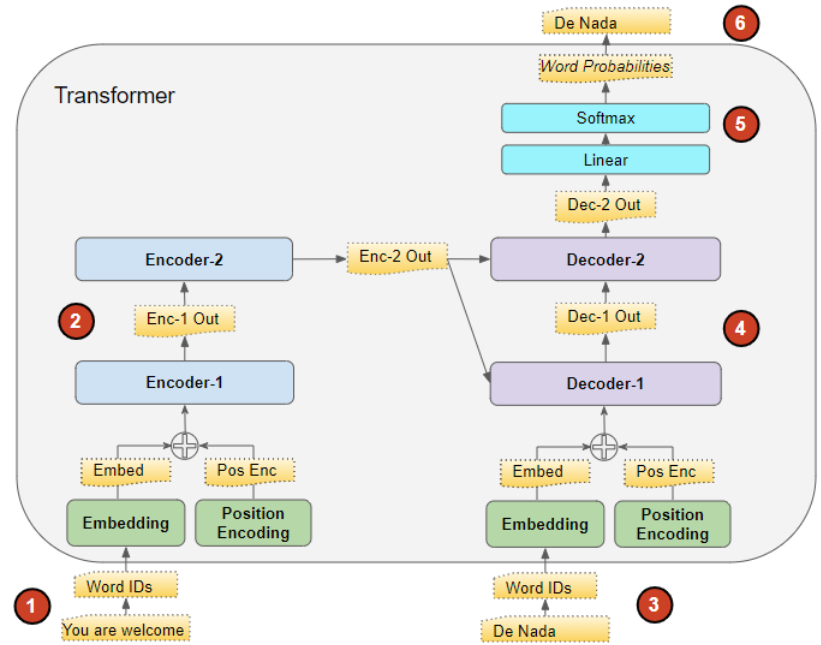
\includegraphics[scale=.3]{Figs/training transformer.png}
\caption{Training the transformer, \href{https://towardsdatascience.com/transformers-explained-visually-part-1-overview-of-functionality-95a6dd460452}{Source}.}
\label{fig:boat1}
\end{figure}
	
}

%%%%%%%%%%%%%%%%%%%%%%%%%%%%%%%%%%%%%%%%%%%%%%%%%%%%%%%%%%%%%%%%%%%%%%%%%%%%%%%%%%%%%%%%%%%%%%%
% \frame{
	
	
% \begin{itemize}
        
% 	\item 
%         Data processing steps by the Transformer:
%         \begin{enumerate}
% 	\item
%         The input sequence is converted into Embeddings (with Position Encoding) and fed to the Encoder.
%         \item
%         The stack of Encoders processes this and produces an encoded representation of the input sequence.
%         \item
%         The target sequence is prepended with a start-of-sentence token, converted into Embeddings (with Position Encoding), and fed to the Decoder.
%         \item
%         The stack of Decoders processes this along with the Encoder stack’s encoded representation to produce an encoded representation of the target sequence.
%         \item
%         The Output layer converts it into word probabilities and the final output sequence.
%         \item
%         The Transformer’s Loss function compares this output sequence with the target sequence from the training data. This loss is used to generate gradients to train the Transformer during back-propagation.
%         \end{enumerate}

% \end{itemize}	
	
% }

%%%%%%%%%%%%%%%%%%%%%%%%%%%%%%%%%%%%%%%%%%%%%%%%%%%%%%%%%%%%%%%%%%%%%%%%%%%%%%%%%%%%%%%%%%%%%%%
\frame{\frametitle{Inference}
	
	
\begin{itemize}
        
	\item 
        During Inference, we have only the input sequence.
         
        \item \vspace{3pt}
        The goal of the Transformer is to produce the target sequence from the input sequence alone.

\end{itemize}	

\begin{figure}
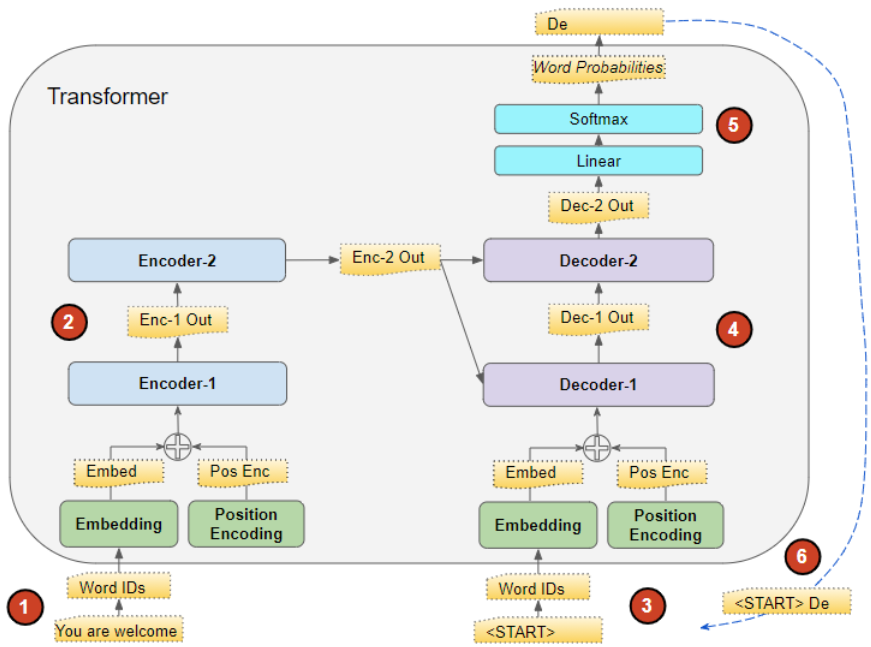
\includegraphics[scale=.35]{Figs/Inference.png}
\caption{Schematic of inference process after first timestamp, \href{https://towardsdatascience.com/transformers-explained-visually-part-1-overview-of-functionality-95a6dd460452}{Source}.}
\label{fig:boat1}
\end{figure}
	
}

%%%%%%%%%%%%%%%%%%%%%%%%%%%%%%%%%%%%%%%%%%%%%%%%%%%%%%%%%%%%%%%%%%%%%%%%%%%%%%%%%%%%%%%%%%%%%%%
% \frame{
	
	
% \begin{itemize}
        
% 	\item 
%         Data processing steps by the Transformer:
%         \begin{enumerate}
% 	\item
%         The input sequence is converted into Embeddings (with Position Encoding) and fed to the Encoder.
%         \item
%         The stack of Encoders processes this and produces an encoded representation of the input sequence.
%         \item
%         Instead of the target sequence, we use an empty sequence with only a start-of-sentence token.
%         \item
%         The stack of Decoders processes this along with the Encoder stack’s encoded representation to produce an encoded representation of the target sequence.
%         \item
%         The Output layer converts it into word probabilities and produces an output sequence.
%         \item
%         We take the last word of the output sequence as the predicted word. That word is now filled into the second position of our Decoder input sequence, which now contains a start-of-sentence token and the first word.
%         \item
%         Go back to step 3. As before, feed the new Decoder sequence into the model. Then take the second word of the output and append it to the Decoder sequence.
%         \end{enumerate}

% \end{itemize}	
	
% }

%%%%%%%%%%%%%%%%%%%%%%%%%%%%%%%%%%%%%%%%%%%%%%%%%%%%%%%%%%%%%%%%%%%%%%%%%%%%%%%%%%%%%%%%%%%%%%%
\frame{\frametitle{Teacher Forcing}
	
	
\begin{itemize}
        
	\item 
        The approach of feeding the target sequence to the Decoder during training is known as Teacher Forcing.
         
        \item \vspace{3pt}
        During training, we could have used the same approach that is used during inference. But there are two major problem:
        \begin{itemize}
	\item 
         The looping cause training to take\tc{keywords}{much}longer. 
         \item \vspace{2pt}
         The looping also makes it\tc{keywords}{harder to train}the model. The model would have to predict the second word based on a potentially erroneous first predicted word, and so on.
        \end{itemize}

        \item \vspace{3pt}
        Instead, by feeding the target sequence to the Decoder, we are giving it a hint, so to speak, just like a Teacher would.

        \item \vspace{3pt}
        In addition, the Transformer is able to output all the words in parallel without looping, which greatly speeds up training.
        

\end{itemize}	

	
}

%%%%%%%%%%%%%%%%%%%%%%%%%%%%%%%%%%%%%%%%%%%%%%%%%%%%%%%%%%%%%%%%%%%%%%%%%%%%%%%%%%%%%%%%%%%%%%%
\frame{\frametitle{Loss Function}
	
	
\begin{itemize}        
	\item 
        During training, we use a loss function such as cross-entropy loss to compare the generated output\tc{keywords}{probability distribution}to the target sequence.

        \item \vspace{3pt}
        The probability distribution gives the probability of each word occurring in that position.

        \item \vspace{3pt}
        As usual, the loss is used to compute gradients to train the Transformer via\tc{keywords}{backpropagation}.
\end{itemize}

\vspace{3pt}

\begin{figure}
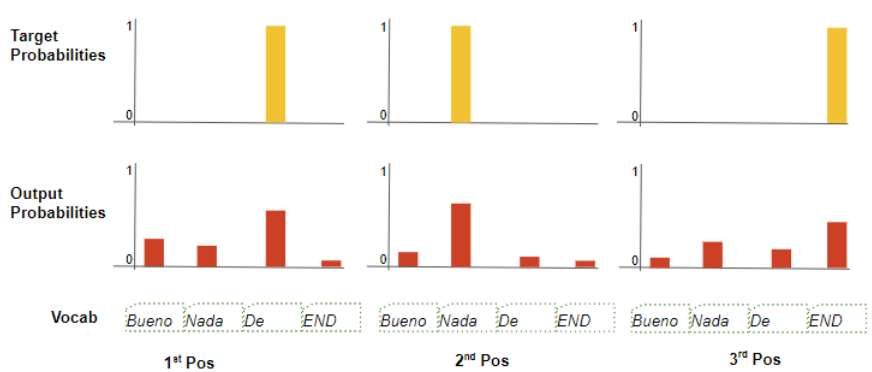
\includegraphics[scale=.45]{Figs/loss function.png}
\caption{The loss function that is used for Transformers, \href{https://towardsdatascience.com/transformers-explained-visually-part-2-how-it-works-step-by-step-b49fa4a64f34}{Source}.}
\label{fig:boat1}
\end{figure}

	
}

%%%%%%%%%%%%%%%%%%%%%%%%%%%%%%%%%%%%%%%%%%%%%%%%%%%%%%%%%%%%%%%%%%%%%%%%%%%%%%%%%%%%%%%%%%%%%%%
\frame{\frametitle{Transformers in Practice}
	
	
\begin{itemize}        
	\item 
        Transformer Classification architecture: one of its examples is in Sentiment Analysis.
\end{itemize}
\vspace{3pt}

\begin{figure}
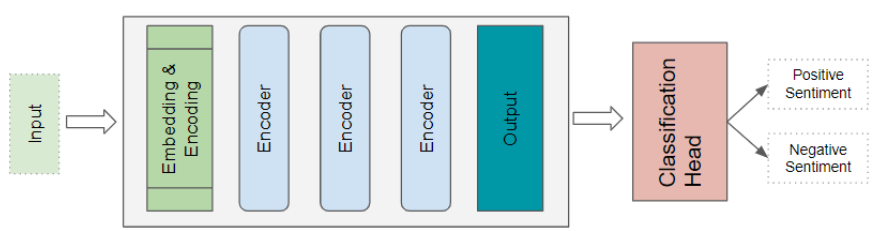
\includegraphics[scale=.4]{Figs/Transformer classify.png}
\caption{\href{https://towardsdatascience.com/transformers-explained-visually-part-1-overview-of-functionality-95a6dd460452}{Source}}
\label{fig:boat1}
\end{figure}

\vspace{3pt}
\begin{itemize}        
	\item 
        Transformer Language Model architecture: one of its examples is generating new text by predicting sentences that would follow a given text as input.
\end{itemize}
\begin{figure}
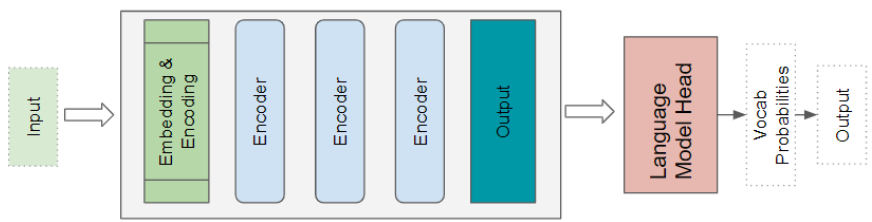
\includegraphics[scale=.4]{Figs/Transformer model head.png}
\caption{\href{https://towardsdatascience.com/transformers-explained-visually-part-1-overview-of-functionality-95a6dd460452}{Source}}
\label{fig:boat1}
\end{figure}
	
}

%%%%%%%%%%%%%%%%%%%%%%%%%%%%%%%%%%%%%%%%%%%%%%%%%%%%%%%%%%%%%%%%%%%%%%%%%%%%%%%%%%%%%%%%%%%%%%%
\frame{\frametitle{Why Transformers instead of RNNs?}
	
	
\begin{itemize}        
	\item 
        RNNs and their relatives, LSTMs and GRUs had two main limitations:
        \begin{itemize}        
	\item
         It was challenging to deal with\tc{keywords}{long-range dependencies}between words that were spread far apart in a long sentence.
         \item \vspace{2pt}
         They process the input sequence sequentially\tc{keywords}{one word at a time}, which means that it cannot do the computation for time-step $t$ until it has completed the computation for time-step $t — 1$.
        \end{itemize}
\end{itemize}
\vspace{3pt}

\begin{figure}
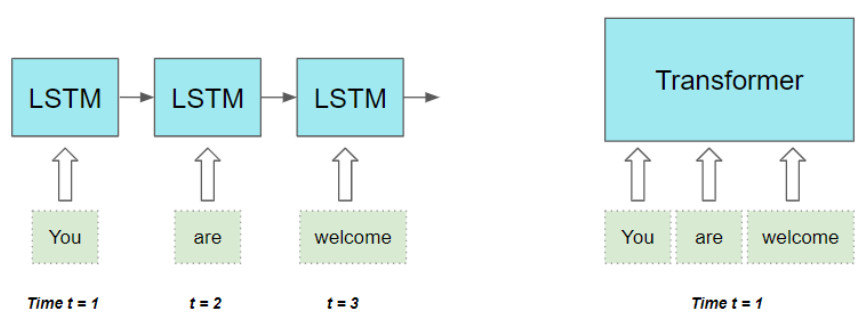
\includegraphics[scale=.4]{Figs/LSTM vs Transformers.png}
\caption{Transformers unlike LSTMs process the words in parallel, \href{https://towardsdatascience.com/transformers-explained-visually-part-1-overview-of-functionality-95a6dd460452}{Source}.}
\label{fig:boat1}
\end{figure}

	
}

%%%%%%%%%%%%%%%%%%%%%%%%%%%%%%%%%%%%%%%%%%%%%%%%%%%%%%%%%%%%%%%%%%%%%%%%%%%%%%%%%%%%%%%%%%%%%%%
\frame{\frametitle{Position Encoding}
	
	
\begin{itemize}        
	\item 
        Transformers don’t use RNNs and all words in a sequence are input in parallel.
        \item \vspace{3pt}
        This is its major advantage over the RNN architecture, but it means that the\tc{keywords}{position information}is lost, and has to be added back in separately.
        \item \vspace{3pt}
        The Position Encoding is computed\tc{keywords}{independently}of the input sequence. 
        \item \vspace{3pt}
        These are\tc{keywords}{fixed values}that depend only on the max length of the sequence. These constants are computed as follows:
        $$PE_{(pos, 2i)} = sin(\frac{pos}{10000^{2i/d_{model}}})$$
        $$PE_{(pos, 2i+1)} = cos(\frac{pos}{10000^{2i/d_{model}}})$$

        where, 
        \begin{itemize}        
	\item 
        $pos$ is the position of the word in the sequence.
        \item \vspace{2pt}
        $d_{model}$ is the length of the encoding vector
        \item \vspace{2pt}
        $i$ is the index value into this vector.
        \end{itemize}
        
\end{itemize}	
}

%%%%%%%%%%%%%%%%%%%%%%%%%%%%%%%%%%%%%%%%%%%%%%%%%%%%%%%%%%%%%%%%%%%%%%%%%%%%%%%%%%%%%%%%%%%%%%%
\frame{\frametitle{Bahdanau’s Attention}

\begin{itemize}   
        \item
        We can think of the google translate as a perfect practice for the Bahdanau’s Attention !
	\item \vspace{4pt}
        The related paper \href{https://www.bing.com/search?q=Neural+Machine+Translation+by+Jointly+Learning+to+Align+and+Translate&cvid=dcb5b37cee4d4bdca5f6db9975e1dfa7&aqs=edge..69i57j69i59i450l8...8.299j0j4&FORM=ANAB01&PC=ASTS}{"Neural Machine Translation by Jointly Learning to Align and Translate"}, propose to build the encoder representation each time a word is decoded in the decoder.
        \item \vspace{4pt}
        This dynamic representation will depend on the parts of the input sentence most relevant to the current decoded word.
        
\end{itemize}
	
}

%%%%%%%%%%%%%%%%%%%%%%%%%%%%%%%%%%%%%%%%%%%%%%%%%%%%%%%%%%%%%%%%%%%%%%%%%%%%%%%%%%%%%%%%%%%%%%%
\frame{

Encoder for the Bahdanau’s Attention:
\vspace{6pt}
\begin{itemize}   
        \item
        A RNN takes the present input $x_t$ and the previous hidden state $h_{t-1}$ to model the present hidden state $h_t$.
	\item \vspace{3pt}
        For the encoder, the authors have suggested a Bidirectional RNN.
        \item \vspace{3pt}
        In a Bidirectional RNN, RNN will provide two sets of hidden states, the forward $\overrightarrow{h_t}$ and the backward $\overleftarrow{h_t}$ hidden states.
        \item \vspace{3pt}
        The authors suggest that concatenating the two states gives a richer and better representation $h_t = [\overrightarrow{h_t};\overleftarrow{h_t}]$
        
\end{itemize}
	
}

%%%%%%%%%%%%%%%%%%%%%%%%%%%%%%%%%%%%%%%%%%%%%%%%%%%%%%%%%%%%%%%%%%%%%%%%%%%%%%%%%%%%%%%%%%%%%%%
\frame{

Decoder for the Bahdanau’s Attention:
\vspace{6pt}
\begin{itemize}   
        \item
        The equation below is of the conditional probability, which needs to be\tc{keywords}{maximized}for the decoder to translate properly.
        $$P(y_i|y_{<\text{i}}, c_i)=\text{RNN}(y_{i-1},s_{i-1},c_i)$$
        
        where $s$ is the hidden state for the decoder and $c_i$ is a newly built context vector for each step.
	\item \vspace{3pt}
        Each context vector depends on the relevant information from which the source sentence is attended.
        \item \vspace{3pt}
        But how important is $h_{t}$ for $s_{t}$? $\longrightarrow$ we need to apply a softmax on the unnormalized importance.
        
\end{itemize}
	
}

%%%%%%%%%%%%%%%%%%%%%%%%%%%%%%%%%%%%%%%%%%%%%%%%%%%%%%%%%%%%%%%%%%%%%%%%%%%%%%%%%%%%%%%%%%%%%%%
\frame{

\begin{figure}
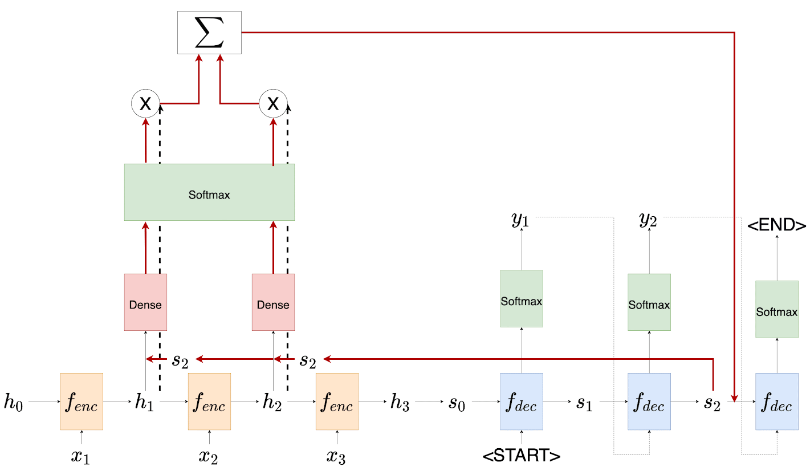
\includegraphics[scale=.6]{Figs/buhad Attention.png}
\caption{Neural machine translation with Bahdanau’s attention, \href{https://pyimagesearch.com/2022/08/22/neural-machine-translation-with-bahdanaus-attention-using-tensorflow-and-keras/}{Source}.}
\label{fig:boat1}
\end{figure}
	
}

%%%%%%%%%%%%%%%%%%%%%%%%%%%%%%%%%%%%%%%%%%%%%%%%%%%%%%%%%%%%%%%%%%%%%%%%%%%%%%%%%%%%%%%%%%%%%%%
\frame{\frametitle{Luong’s Attention}

\begin{itemize}   
        \item
        In the related paper \href{https://arxiv.org/abs/1508.04025}{"Effective Approaches to Attention-Based Neural Machine Translation"}, Luong et al. provide more effective approaches to building attention.
	\item \vspace{4pt}
        The basic intuition behind attention is still the same as before.
        \item \vspace{4pt}
        Luong et al. suggested subtle changes to Bahdanau et al. work to break through the limitations of the old architecture.
        
\end{itemize}
	
}

%%%%%%%%%%%%%%%%%%%%%%%%%%%%%%%%%%%%%%%%%%%%%%%%%%%%%%%%%%%%%%%%%%%%%%%%%%%%%%%%%%%%%%%%%%%%%%%
\frame{

\begin{figure}
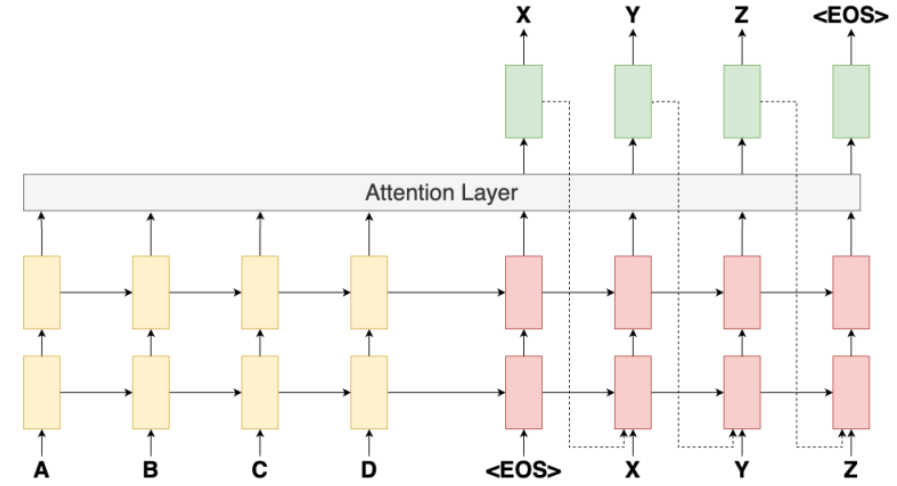
\includegraphics[scale=.6]{Figs/Luog Attention.png}
\caption{Diagram of the Luong attention architecture, \href{https://pyimagesearch.com/2022/08/29/neural-machine-translation-with-luongs-attention-using-tensorflow-and-keras/}{Source}.}
\label{fig:boat1}
\end{figure}
	
}

%%%%%%%%%%%%%%%%%%%%%%%%%%%%%%%%%%%%%%%%%%%%%%%%%%%%%%%%%%%%%%%%%%%%%%%%%%%%%%%%%%%%%%%%%%%%%%%
\frame{

Encoder for the Luong’s Attention:
\vspace{6pt}
\begin{itemize}   
        \item
        In this model, authors opt for a\tc{keywords}{unidirectional}(instead of bidirectional as in Bahdanau’s implementation) Recurrent Neural architecture for the encoder.
	\item \vspace{4pt}
        Unidirectional RNNs speed up the computation.
        
\end{itemize}
\vspace{6pt}
Decoder for the Luong’s Attention:
\vspace{6pt}
\begin{itemize}   
        \item
        given the target hidden state, $s_{t}$, and the source-side context vector, $c_{t}$, they employ a simple concatenation layer as follows:
        $$\widetilde{s}_t=tanh(W_c[c_t;s_t])$$
	\item \vspace{4pt}
        The attention vector, $\tilde{s_{t}}$, is then fed through the softmax layer to produce the probability of the next decoder word.
        
\end{itemize}
	
}

%%%%%%%%%%%%%%%%%%%%%%%%%%%%%%%%%%%%%%%%%%%%%%%%%%%%%%%%%%%%%%%%%%%%%%%%%%%%%%%%%%%%%%%%%%%%%%%
\frame{

\begin{figure}
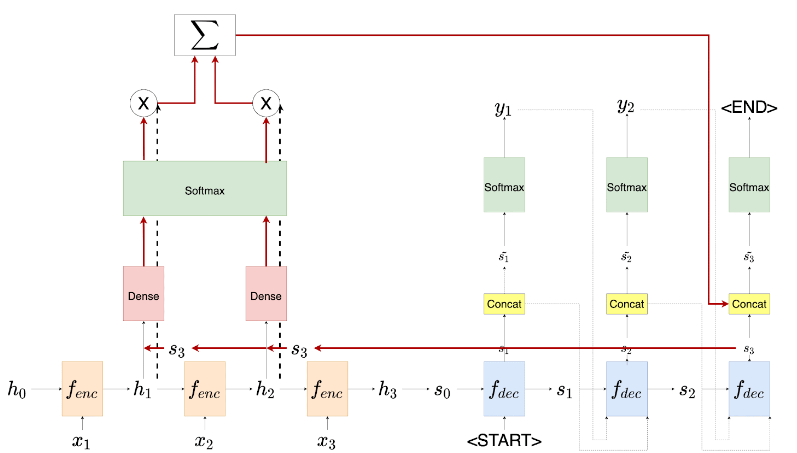
\includegraphics[scale=.6]{Figs/Luog Attention 2.png}
\caption{Neural machine translation with Luong’s attention, \href{https://pyimagesearch.com/2022/08/29/neural-machine-translation-with-luongs-attention-using-tensorflow-and-keras/}{Source}.}
\label{fig:boat1}
\end{figure}
	
}

%%%%%%%%%%%%%%%%%%%%%%%%%%%%%%%%%%%%%%%%%%%%%%%%%%%%%%%%%%%%%%%%%%%%
\frametitle{Final Notes}
\centering
\vspace{50 pt}
\textbf{Thank You!}
\vspace{50pt}

\textbf{Any Question?}
%%%%%%%%%%%%%%%%%%%%%%%%%%%%%%%%%%%%%%%%%%
\end{document}